\documentclass[11pt,a4paper]{article}
\usepackage[utf8]{vietnam}
\usepackage{amsmath,amssymb,mathrsfs}
\usepackage{graphicx}
\usepackage{tikz}
\usepackage{array}
\usepackage[top=1.0cm,bottom=1.8cm,left=1.4cm,right=1.4cm,footskip=0.8cm,headheight=16pt]{geometry}
\usepackage{fancyhdr}
\usepackage{tcolorbox}
\tcbuselibrary{skins}
\usepackage{lastpage}
\usepackage[dethi]{ex_test}
\graphicspath{{../../Hinh_Anh/NH_10/}}

\makeatletter
\@ifundefined{c@bt}{\newcounter{bt}}{}
\makeatother

\pagestyle{fancy}
\fancyhf{}
\renewcommand{\headrulewidth}{0pt}
\renewcommand{\footrulewidth}{0.4pt}
\lfoot{\footnotesize\textsl{Lớp Toán Cô Thúy -- SĐT: 0935.322.328 -- 50/2C Phạm Thị Liên}}
\rfoot{\footnotesize\textsl{Trang \thepage/\pageref{LastPage} -- Mã đề 494}}
\setlength{\parskip}{1pt}
\setlength{\parindent}{0pt}

\begin{document}

\noindent
\begin{tabular}{|p{6.6cm}|p{6.6cm}|>{\centering\arraybackslash}p{3.2cm}|}
\hline
\begin{minipage}{6.6cm}
\vspace{3pt}
\centering
{\large\bfseries\color{blue!80!black} LỚP TOÁN CÔ THÚY}\\[3pt]
\textbf{SĐT:} 0935.322.328\\[2pt]
\textbf{Địa chỉ:} 50/2C Phạm Thị Liên
\vspace{3pt}
\end{minipage}
&
\multicolumn{2}{p{10.2cm}|}{
\begin{minipage}{10.2cm}
\vspace{3pt}
\centering
{\bfseries\color{red!80!black} KIỂM TRA GIỮA KỲ I -- NĂM HỌC 2025 -- 2026}\\[3pt]
\textbf{Môn: VẬT LÍ, Lớp 10 -- THPT NGUYỄN HUỆ}\\[2pt]
\textit{Thời gian làm bài: 45 phút (Không kể thời gian phát đề)}
\vspace{3pt}
\end{minipage}
} \\
\hline
\rule{0pt}{13pt}Họ và tên thí sinh: \dotfill\rule[-3pt]{0pt}{3pt} &
\rule{0pt}{13pt}Số báo danh: \dotfill\rule[-3pt]{0pt}{3pt} &
\rule{0pt}{13pt}\textbf{Mã đề thi 494}\rule[-3pt]{0pt}{3pt} \\
\hline
\end{tabular}
\vspace{0.1cm}

\vspace{0.15cm}
\begin{flushleft}
	{\color{blue!50!green}\fbox{\fontfamily{qag}\bfseries\selectfont PHẦN I. Câu trắc nghiệm nhiều phương án lựa chọn (3,0 điểm)}}
	\textit{\small (Thí sinh trả lời từ câu 1 đến câu 12. Mỗi câu hỏi thí sinh chỉ chọn một phương án.)}
\end{flushleft}
\setcounter{ex}{0}
\setcounter{bt}{0}

% Câu 1
\begin{ex}
	Một vật rơi tự do, sau $3\text{ s}$ kể từ khi bắt đầu rơi, vận tốc của vật là bao nhiêu? (Lấy $g = 9{,}8\text{ m/s}^2$).
	\choice
	{\True $29{,}4\text{ m/s}$}
	{$4{,}9\text{ m/s}$}
	{$19{,}8\text{ m/s}$}
	{$39{,}2\text{ m/s}$}
	\loigiai{
		Vận tốc của vật rơi tự do từ trạng thái nghỉ sau thời gian $t$ là:\par
		\[v = gt = 9{,}8 \cdot 3 = 29{,}4\text{ m/s}.\]
	}
\end{ex}

% Câu 2
\begin{ex}
	Đối tượng nghiên cứu cốt lõi của Vật lí học tập trung chủ yếu vào
	\choice
	{\True các dạng vận động của vật chất và các dạng năng lượng trong tự nhiên}
	{vật lí nguyên tử và cấu trúc các hạt nhân}
	{các dạng vận động sinh học của phân tử sinh vật và năng lượng sống}
	{các phân môn Cơ học, Nhiệt học, Điện học, Quang học cổ điển}
	\loigiai{
		Đối tượng nghiên cứu của Vật lí học bao gồm các dạng vận động cơ bản của vật chất (cơ, nhiệt, điện, từ, quang, hạt nhân,...) và các dạng năng lượng tương tác giữa chúng trong tự nhiên.\par
	}
\end{ex}

% Câu 3
\begin{ex}
	Trong thí nghiệm đo tốc độ chuyển động thẳng của xe lăn trên máng đỡ, học sinh dùng cảm biến thời gian và thước đo quãng đường. Kết quả đo được: xe đi được quãng đường $s = 0{,}50\text{ m}$ trong thời gian $t = 1{,}25\text{ s}$. Tốc độ trung bình của xe là
	\choice
	{$0{,}25\text{ m/s}$}
	{\True $0{,}40\text{ m/s}$}
	{$0{,}60\text{ m/s}$}
	{$0{,}50\text{ m/s}$}
	\loigiai{
		Tốc độ trung bình của xe lăn:\par
		\[v_{\text{tb}} = \frac{s}{t} = \frac{0{,}50}{1{,}25} = 0{,}40\text{ m/s}.\]
	}
\end{ex}

% Câu 4
\begin{ex}
	Kết luận nào sau đây là \textbf{sai} khi nói về độ dịch chuyển của một vật chuyển động?
	\choice
	{Khi vật chuyển động thẳng, không đổi chiều thì độ lớn của độ dịch chuyển bằng quãng đường đi được ($d = s$)}
	{\True Khi vật chuyển động thẳng, có đổi chiều thì độ lớn của độ dịch chuyển bằng quãng đường đi được ($d = s$)}
	{Độ dịch chuyển được biểu diễn bằng một mũi tên nối vị trí đầu và vị trí cuối của chuyển động}
	{Độ dịch chuyển có thể nhận giá trị dương, âm hoặc bằng $0$}
	\loigiai{
		Khi vật chuyển động thẳng có đổi chiều, quãng đường đi được lớn hơn độ lớn của độ dịch chuyển ($s > d$). Do đó kết luận B là sai.\par
	}
\end{ex}

% Câu 5
\begin{ex}
	Trong thí nghiệm đo gia tốc rơi tự do, học sinh thả một quả bóng nhỏ từ độ cao $h = 1{,}20\text{ m}$. Thời gian rơi trung bình đo được là $t = 0{,}495\text{ s}$. Bỏ qua lực cản không khí. Giá trị gia tốc rơi tự do $g$ gần nhất với giá trị nào sau đây?
	\choice
	{\True $9{,}79\text{ m/s}^2$}
	{$8{,}85\text{ m/s}^2$}
	{$9{,}02\text{ m/s}^2$}
	{$10{,}2\text{ m/s}^2$}
	\loigiai{
		Công thức rơi tự do: $h = \dfrac{1}{2}gt^2 \Rightarrow g = \dfrac{2h}{t^2}$.\par
		\[g = \frac{2 \cdot 1{,}20}{(0{,}495)^2} \approx 9{,}795\text{ m/s}^2 \approx 9{,}79\text{ m/s}^2.\]
	}
\end{ex}

% Câu 6
\begin{ex}
	Hành động nào sau đây vi phạm nguyên tắc an toàn khi làm thí nghiệm thực hành Vật lí?
	\choice
	{Không chạm tay vào các thiết bị điện khi đang hoạt động}
	{\True Chạm tay trực tiếp vào ổ điện, dây dẫn trần hoặc thiết bị điện đang hoạt động khi chưa ngắt nguồn}
	{Sau khi làm xong thí nghiệm phải tắt nguồn điện, rút phích cắm và dọn dẹp nơi làm việc}
	{Chỉ tiến hành thí nghiệm khi có sự cho phép và hướng dẫn của giáo viên}
	\loigiai{
		Chạm tay trực tiếp vào ổ điện, dây dẫn trần hoặc thiết bị chưa ngắt nguồn có nguy cơ gây điện giật nguy hiểm đến tính mạng, vi phạm nghiêm trọng quy tắc an toàn.\par
	}
\end{ex}

% Câu 7
\begin{ex}
	Trong thí nghiệm đo các đại lượng vật lí, để giảm thiểu sai số ngẫu nhiên của phép đo, người ta thường
	\choice
	{\True thực hiện phép đo lặp lại nhiều lần và tính giá trị trung bình}
	{chỉ đo một lần duy nhất để tiết kiệm thời gian}
	{giảm bớt khối lượng của vật làm thí nghiệm}
	{tăng khối lượng của vật làm thí nghiệm}
	\loigiai{
		Sai số ngẫu nhiên xuất hiện do các yếu tố ngẫu nhiên không kiểm soát được. Để giảm sai số ngẫu nhiên, ta cần lặp lại phép đo nhiều lần trong cùng điều kiện và tính giá trị trung bình.\par
	}
\end{ex}

% Câu 8
\begin{ex}
	Một vật chuyển động thẳng nhanh dần đều từ trạng thái nghỉ ($v_0 = 0$). Sau thời gian $4\text{ s}$, vận tốc của vật đạt $10\text{ m/s}$. Gia tốc của chuyển động là
	\choice
	{\True $2{,}5\text{ m/s}^2$}
	{$0{,}5\text{ m/s}^2$}
	{$5\text{ m/s}^2$}
	{$10\text{ m/s}^2$}
	\loigiai{
		Gia tốc của vật:\par
		\[a = \frac{v - v_0}{t} = \frac{10 - 0}{4} = 2{,}5\text{ m/s}^2.\]
	}
\end{ex}

% Câu 9
\begin{ex}
	Vận tốc tức thời là một đại lượng vectơ đặc trưng cho
	\choice
	{\True độ nhanh chậm và hướng chuyển động của vật tại một thời điểm xác định}
	{độ nhanh chậm của chuyển động, luôn nhận giá trị không âm}
	{quãng đường vật đi được trong một đơn vị thời gian}
	{chiều biến thiên của gia tốc}
	\loigiai{
		Vận tốc tức thời $\vec{v}$ là đại lượng vectơ, cho biết mức độ nhanh chậm và hướng chuyển động của vật tại thời điểm quan sát.\par
	}
\end{ex}

% Câu 10
\begin{ex}
	Cặp đồ thị nào trong hình vẽ dưới đây biểu diễn đặc trưng cho chuyển động thẳng đều?
	\begin{center}
		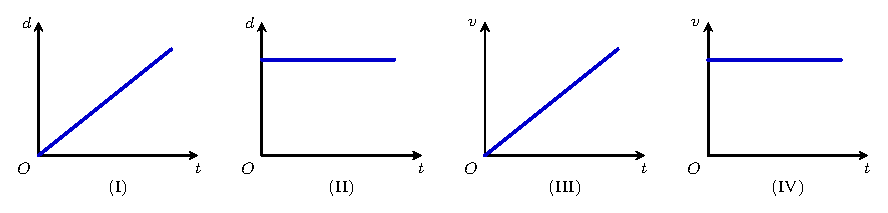
\includegraphics[width=12.0cm]{fig_cau10.pdf}
	\end{center}
	\choice
	{(II) và (III)}
	{\True (I) và (IV)}
	{(I) và (III)}
	{(II) và (IV)}
	\loigiai{
		-- Trong chuyển động thẳng đều, $d = vt$ nên đồ thị $d - t$ là đường thẳng qua gốc tọa độ $\Rightarrow$ Đồ thị (I).\par
		-- Vận tốc không đổi theo thời gian ($v = \text{const}$) nên đồ thị $v - t$ là đường thẳng song song trục thời gian $\Rightarrow$ Đồ thị (IV).\par
		Vậy cặp đồ thị đúng là (I) và (IV).\par
	}
\end{ex}

% Câu 11
\begin{ex}
	Gia tốc của một chuyển động thẳng biến đổi là đại lượng đặc trưng cho
	\choice
	{\True sự biến thiên nhanh hay chậm của vận tốc theo thời gian}
	{độ lớn của vận tốc tức thời}
	{tổng chiều dài quãng đường vật đi được}
	{hướng chuyển động của vật}
	\loigiai{
		Gia tốc $\vec{a} = \dfrac{\Delta \vec{v}}{\Delta t}$ đặc trưng cho tốc độ biến thiên của vectơ vận tốc theo thời gian.\par
	}
\end{ex}

% Câu 12
\begin{ex}
	Sai số tỉ đối $\delta A$ của phép đo đại lượng vật lí $A$ được xác định theo công thức nào?
	\choice
	{\True $\delta A = \dfrac{\Delta A}{\overline{A}} \cdot 100\%$}
	{$\delta A = |\overline{A} - A|$}
	{$\delta A = \Delta A \cdot 100\%$}
	{$\delta A = \dfrac{A}{\overline{A}} \cdot 100\%$}
	\loigiai{
		Sai số tỉ đối là tỉ số phần trăm giữa sai số tuyệt đối toàn phần $\Delta A$ và giá trị trung bình $\overline{A}$: $\delta A = \dfrac{\Delta A}{\overline{A}} \cdot 100\%$.\par
	}
\end{ex}

\vspace{0.15cm}
\begin{flushleft}
	{\color{blue!50!green}\fbox{\fontfamily{qag}\bfseries\selectfont PHẦN II. Câu trắc nghiệm đúng sai (2,0 điểm)}}
	\textit{\small (Thí sinh trả lời từ câu 1 đến câu 2. Trong mỗi ý a), b), c), d) ở mỗi câu, thí sinh chọn đúng hoặc sai.)}
\end{flushleft}
\setcounter{ex}{0}
\setcounter{bt}{0}

% Phần II Câu 1
\begin{ex}
	Một vật chuyển động thẳng đều dọc theo trục $Ox$.
	\choiceTF[t]
	{\True Vectơ vận tốc của vật luôn cùng hướng với hướng chuyển động của vật.}
	{\True Vận tốc đại số có thể mang dấu âm hoặc dương, còn tốc độ luôn không âm.}
	{Nếu vật chuyển động về phía đầu tàu với vận tốc $2\text{ m/s}$ so với sàn tàu, đồng thời đoàn tàu chạy với vận tốc $10\text{ m/s}$ so với đường ray (cùng chiều về hướng Đông), thì vận tốc của vật đối với mặt đường có độ lớn bằng $8\text{ m/s}$.}
	{\True Tốc độ tức thời cho biết mức độ nhanh hay chậm của chuyển động tại thời điểm xét.}
	\loigiai{
		{\color{green!50!black}\textbf{a) Đúng.}} Vectơ vận tốc $\vec{v}$ luôn cùng hướng với chiều chuyển động của vật.\par
		{\color{green!50!black}\textbf{b) Đúng.}} Vận tốc $v$ là đại lượng đại số phụ thuộc chiều dương đã chọn, còn tốc độ là độ lớn của vận tốc nên $v_{\text{tốc độ}} = |\vec{v}| \ge 0$.\par
		{\color{red!80!black}\textbf{c) Sai.}} Hai chuyển động cùng chiều nên áp dụng công thức cộng vận tốc: $v = v_1 + v_2 = 2 + 10 = 12\text{ m/s} \ne 8\text{ m/s}$.\par
		{\color{green!50!black}\textbf{d) Đúng.}} Tốc độ tức thời đặc trưng cho mức độ nhanh chậm của chuyển động tại từng thời điểm.\par
	}
\end{ex}

% Phần II Câu 2
\begin{ex}
	Một chất điểm chuyển động dọc theo một đường thẳng từ điểm $A$ đến điểm $B$.
	\choiceTF[t]
	{Khi chất điểm đi từ $A$ đến $B$ rồi quay về lại $A$, quãng đường đi được bằng $0$.}
	{Độ lớn của độ dịch chuyển luôn luôn bằng quãng đường vật đi được trong mọi trường hợp.}
	{\True Quãng đường đi được của chất điểm luôn lớn hơn hoặc bằng độ lớn độ dịch chuyển ($s \ge d$).}
	{\True Nếu chất điểm đi thẳng từ $A$ đến $B$ ($AB = 5\text{ m}$) rồi quay ngược lại điểm $C$ ($BC = 2\text{ m}$), thì độ lớn độ dịch chuyển của vật bằng $3\text{ m}$.}
	\loigiai{
		{\color{red!80!black}\textbf{a) Sai.}} Khi quay về vị trí ban đầu $A$, độ dịch chuyển bằng $0$ nhưng quãng đường $s = AB + BA = 2AB \ne 0$.\par
		{\color{red!80!black}\textbf{b) Sai.}} Độ lớn độ dịch chuyển chỉ bằng quãng đường khi vật chuyển động thẳng và không đổi chiều.\par
		{\color{green!50!black}\textbf{c) Đúng.}} Độ dịch chuyển là khoảng cách thẳng nối điểm đầu và điểm cuối nên luôn có $s \ge d$.\par
		{\color{green!50!black}\textbf{d) Đúng.}} Vật đi từ $A$ đến $B$ rồi quay lại $C$: điểm đầu là $A$, điểm cuối là $C$ nên độ dịch chuyển $d = AC = AB - BC = 5 - 2 = 3\text{ m}$.\par
	}
\end{ex}

\vspace{0.15cm}
\begin{flushleft}
	{\color{blue!50!green}\fbox{\fontfamily{qag}\bfseries\selectfont PHẦN III. Câu trắc nghiệm trả lời ngắn (2,0 điểm)}}
	\textit{\small (Thí sinh trả lời từ câu 1 đến câu 4.)}
\end{flushleft}
\setcounter{ex}{0}
\setcounter{bt}{0}

% Phần III Câu 1
\begin{ex}
	Một vật đi được quãng đường $0{,}6\text{ km}$ trong thời gian $2\text{ phút}$. Tốc độ trung bình của vật là bao nhiêu $\text{m/s}$?
	\par\shortans[oly]{5}
	\loigiai{
		Đổi đơn vị: $s = 0{,}6\text{ km} = 600\text{ m}$, $t = 2\text{ phút} = 120\text{ s}$.\par
		\[v_{\text{tb}} = \frac{s}{t} = \frac{600}{120} = 5\text{ m/s}.\]
	}
\end{ex}

% Phần III Câu 2
\begin{ex}
	Một ô tô đi thẳng từ $A$ đến $B$ cách $A$ một khoảng $300\text{ m}$, sau đó quay đầu chạy về $C$ cách $A$ một khoảng $100\text{ m}$ ($C$ nằm giữa $A$ và $B$). Tổng quãng đường ô tô đã đi được là bao nhiêu mét?
	\par\shortans[oly]{500}
	\loigiai{
		Quãng đường chặng 1: $s_1 = AB = 300\text{ m}$.\par
		Quãng đường chặng 2: $s_2 = BC = AB - AC = 300 - 100 = 200\text{ m}$.\par
		\[s = s_1 + s_2 = 300 + 200 = 500\text{ m}.\]
	}
\end{ex}

% Phần III Câu 3
\begin{ex}
	Một ô tô đang chuyển động thẳng đều với vận tốc $8\text{ m/s}$ thì tăng tốc chuyển động thẳng nhanh dần đều. Sau $16\text{ s}$, vận tốc của xe đạt $12\text{ m/s}$. Quãng đường ô tô đi được kể từ lúc tăng tốc cho đến khi đạt vận tốc $16\text{ m/s}$ là bao nhiêu mét?
	\par\shortans[oly]{384}
	\loigiai{
		Gia tốc của xe: $a = \dfrac{v_1 - v_0}{t_1} = \dfrac{12 - 8}{16} = 0{,}25\text{ m/s}^2$.\par
		Áp dụng hệ thức độc lập thời gian từ lúc $v_0 = 8\text{ m/s}$ đến $v_2 = 16\text{ m/s}$:\par
		\[v_2^2 - v_0^2 = 2as \Rightarrow 16^2 - 8^2 = 2 \cdot 0{,}25 \cdot s \Rightarrow 192 = 0{,}5s \Rightarrow s = 384\text{ m}.\]
	}
\end{ex}

% Phần III Câu 4
\begin{ex}
	Thả một vật rơi tự do từ độ cao $h$ so với mặt đất. Thời gian rơi chạm đất là $2\text{ s}$. Lấy $g = 9{,}8\text{ m/s}^2$. Độ cao $h$ bằng bao nhiêu mét?
	\par\shortans[oly]{19,6}
	\loigiai{
		\[h = \frac{1}{2}gt^2 = \frac{1}{2} \cdot 9{,}8 \cdot 2^2 = 19{,}6\text{ m}.\]
	}
\end{ex}

\vspace{0.15cm}
\begin{flushleft}
	{\color{blue!50!green}\fbox{\fontfamily{qag}\bfseries\selectfont PHẦN IV. Tự luận (3,0 điểm)}}
	\textit{\small (Thí sinh trình bày lời giải từ câu 1 đến câu 3.)}
\end{flushleft}
\setcounter{ex}{0}
\setcounter{bt}{0}

% Phần IV Câu 1
\begin{ex}
	Một chiếc xe máy chuyển động thẳng có đồ thị độ dịch chuyển -- thời gian $(d - t)$ như hình bên.
	\par \textbf{a)} Nêu tính chất chuyển động của xe máy. \par \textbf{b)} Tính vận tốc của xe máy.
	\begin{center}
		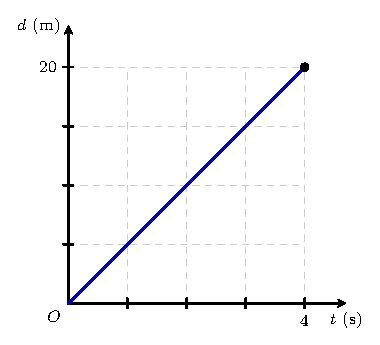
\includegraphics[width=6.5cm]{fig_cau19.pdf}
	\end{center}
	\loigiai{
		\textbf{a)} Đồ thị $(d - t)$ là đường thẳng đi qua gốc tọa độ $O$, chứng tỏ độ dịch chuyển tăng tỉ lệ thuận với thời gian theo hàm bậc nhất. Do đó, xe máy chuyển động thẳng đều theo chiều dương.\par
		\textbf{b)} Từ đồ thị, tại thời điểm $t = 4\text{ s}$ xe có độ dịch chuyển $d = 20\text{ m}$. Vận tốc của xe là:\par
		\[v = \frac{d}{t} = \frac{20}{4} = 5\text{ m/s}.\]
	}
\end{ex}

% Phần IV Câu 2
\begin{ex}
	Từ đỉnh một vách núi thẳng đứng, một người thả rơi tự do một hòn đá nhỏ xuống đáy vực sâu. Sau thời gian $9\text{ s}$ kể từ lúc thả, người đó nghe thấy tiếng đá chạm vào đáy vực. Biết vận tốc truyền âm trong không khí là $320\text{ m/s}$, lấy $g = 9{,}8\text{ m/s}^2$. Tính độ cao của đỉnh vách núi so với đáy vực (làm tròn đến hàng đơn vị mét).
	\loigiai{
		Gọi $h$ là độ cao của vách núi. Thời gian $9\text{ s}$ gồm hai giai đoạn:\par
		-- Thời gian hòn đá rơi tự do xuống đáy vực: $t_1 = \sqrt{\dfrac{2h}{g}} = \sqrt{\dfrac{h}{4{,}9}}$.\par
		-- Thời gian âm thanh truyền từ đáy vực lên tai người: $t_2 = \dfrac{h}{v_{\text{âm}}} = \dfrac{h}{320}$.\par
		Phương trình tổng thời gian:\par
		\[t_1 + t_2 = 9 \Rightarrow \sqrt{\frac{h}{4{,}9}} + \frac{h}{320} = 9.\]
		Đặt $X = \sqrt{h} \ge 0$, phương trình trở thành:\par
		\[\frac{1}{320}X^2 + \frac{1}{\sqrt{4{,}9}}X - 9 = 0.\]
		Giải phương trình bậc hai ta được nghiệm dương: $X \approx 17{,}49 \Rightarrow h = X^2 \approx 306\text{ m}$.\par
	}
\end{ex}

% Phần IV Câu 3
\begin{ex}
	Một vật bắt đầu chuyển động thẳng nhanh dần đều từ trạng thái nghỉ ($v_0 = 0$). Sau $3\text{ s}$, vật đi được quãng đường $9\text{ m}$. Hãy xác định:
	\par \textbf{a)} Gia tốc của vật. \par \textbf{b)} Thời gian kể từ lúc bắt đầu chuyển động để vật đạt vận tốc $15\text{ m/s}$.
	\loigiai{
		\textbf{a)} Quãng đường vật đi được: $s = \dfrac{1}{2}at^2 \Rightarrow 9 = \dfrac{1}{2}a \cdot 3^2 = 4{,}5a \Rightarrow a = 2\text{ m/s}^2$.\par
		\textbf{b)} Vận tốc tại thời điểm $t$: $v = at \Rightarrow 15 = 2t \Rightarrow t = 7{,}5\text{ s}$.\par
	}
\end{ex}

\vspace{0.4cm}
\begin{center}
	\textbf{--------- HẾT ---------}
\end{center}

\end{document}
